\chapter{Das AUVSI Projekt}\label{cha:Das AUVSI Projekt}

\section{Historie und Intention des AUVSI SUAS-Wettbewerbs}
Seit 2002 findet jährlich der AUVSI (Association for Unmanned Vehicle Systems International) SUAS (Student Unmanned Aerial Systems Competition)-Wettbewerb in den USA statt.

Hieran hat die Hochschule in den Jahren 2015 und 2016 erfolgreich teilgenommen. Bereits im Jahr 2014 gab es die ersten Anstrengungen ein für diesen Wettbewerb passende Flugplattform zu entwickeln. Leider war dies zu diesem Zeitpunkt noch nicht von Erfolg gekrönt. Detaillierte Informationen hierzu können der Diplomarbeit von Herrn Dipl. Ing. Fabian Meilinger entnommen werden \cite{Meiling}.

Die Hauptintention des Wettbewerbs ist neben der Förderung des Interesses an unbemannten Flugsystemen (Unmanned Aerial Systems - UAS), Studenten für solche Technologien zu begeistern und für die Industrie zu gewinnen. Aufgabe der Studenten im Wettbewerb ist es, ein unbemanntes Flugsystem zu entwerfen, das autonom fliegen und navigieren kann, notwendige Komponenten zu integrieren und vorzuführen. Zusätzlich muss die Umgebung über integrierte Sensoren erfasst und nach spezifischen Objekten durchsucht werden können. Des Weiteren müssen die Studenten einen detaillierten Bericht erstellen.

Der Wettbewerb findet auf dem "Webster Field der Patuxent River Naval Air Station" (NAS) im St. Mary's County, Maryland, statt dem Stützpunkt der "Unmanned Aircraft Systems Test Directorate" der US Navy.

Der Hauptaugenmerk des Wettbewerbs liegt auf der Verwendung eines autonomen Flugsystems. Je automatisierter das System die Aufgaben erfüllen kann, desto mehr Punkte erhält das Team.

Die während des Wettbewerbs gestellten Aufgaben sollen eine reale Mission emulieren. Da die Aufgaben die wesentlichen Interessenfelder der Industrie widerspiegeln sollen, werden diese jährlich modifiziert und variiert.

\clearpage

Dabei fokusiert sich der Wettbewerb immer auf die folgenden drei Aufgabenfelder \cite{AUVSIrules}:
\begin{itemize}
\item Voraberstellung eines technischen Berichts mit Beschreibung des Flugsystems und seiner Komponenten.
\item Flugbereitschaftspräsentation in der das Team die Einsatzfähigkeit seines Systems anhand der durchgeführten Flugversuche darlegt. 
\item Missionsdurchführung bei der die ausgewählten und im Bericht beschriebenen Aufgabenstellungen bewältigt werden sollen. Dazu gehören zum Beispiel:

\begin{itemize}

\item \textbf{Kommunikations- und Interaktionsfähigkeit:} Das UAS lädt sich die Missionsdetails von einem beritgestellten Server herunter, lädt die Telemetriedaten des Flugzeuges in Echtzeit auf diesen Server hoch und leitet die Missionsergebnisse zu einem externen System weiter. Dort werden die Ergebnisse bewertet.

\item \textbf{Autonomer Flug:} Das UAV startet autonom und darf nur einen gegebenen Bereich befliegen, in dem es mehrere Wegpunkte passieren und seine Missionen bewältigen muss.

\item \textbf{Hindernisvermeidung:} Das UAS soll autonom stationäre bzw. bewegliche Hindernisse umfliegen.

\item \textbf{Objekterkennung:} Das UAS soll Bilder eines gegebenen Suchbereichs aufnehmen und darin deponierte Objekte (meist Buchstaben) erkennen, deren Eigenschaften wie Form und Farbe im Vorhinein bekannt gegeben sind. Diese sollen lokalisiert (GPS-Position) und klassifiziert werden.

\item \textbf{Luftfracht:} Das UAS soll autonom ein Nutzlastobjekt abwerfen, welches an einer vorgegebenen GPS-Position unbeschädigt landen soll.

\end{itemize}

\end{itemize}



\section{Das Studentische AUVSI Team}
Erste Ideen an dem Wettbewerb teilzunehmen entstanden nach den Erfahrungen von Fabian Meilinger während seines Auslandssemesters an der MB Riddle University, wo bereits seit längerem ein Team beim AUVSI SUAS-Wettbewerb antrat. 
Hieraus formierte sich 2014 erstmals ein studentisches Team unter der Leitung von Prof. Karl Siebold. Dieses konnte erste Erkenntnisse für ein Wettbewerb geeignetes Flugsystem sammeln. 

In Ermangelung eines ausreichend zuverlässigen Betriebes des Flugzeugs war eine Teilnahme am Wettbewerb 2014 noch nicht möglich.

Im folgenden Jahr wurde erstmals ein Flugzeug eigenständig vom Team entwickelt und gefertigt. Federführend war dabei Herr Dipl.Ing. Sebastian Donner, der als Laboringenieur die gesamte Entwicklung fachlich betreut und geleitet hat. Mit diesem Flugzeug gelang die erste Teilnahme am Wettbewerb. Dabei wurde der achte Platz in der Gesamtwertung erreicht und der siebte Platz bei der Missionsdurchführung, die beste Platzierung, die je ein Team bei der ersten Teilnahme erreicht hat.   

Für 2016 wurde das identische Konzept angewendet mit Weiterentwicklung des Flugzeugs von 2015. 2016 belegte das Team den 7. Platz in der Gesamtwertung und gewann den 'Dr. Arthur Reyes Safety Award'.

2017 fokussierte sich das Team auf ein anderes Forschungsprojekt, weshalb keine Teilnahme am Wettbewerb möglich war. Für die Saison 2018 laufen aktuell erste Vorentwicklungen.

\section{Ecuador-Projekt (Geschichte und Hintergrund)}

\colorbox{red}{!!! Fehlt noch w i c h t i g - Niclas!!!} \cite{Niclas}

\begin{figure}[H]
\centering
\includegraphics[width=0.9\textwidth]{bilder/Fotos/Ecuador_2015_Gruppenbild.jpg} 
\caption{Die Forschungsgruppe in Sharametsa} 
\label{Die Forschungsgruppe in Sharametsa}
\end{figure}

\clearpage

\section{(Entwicklungsgeschichte) Bisherige Flugzeuge}

Vorwiegend für das UAV Projekts sind im Labor für Systemtechnik verschiedenste Flugplattformen betrieben worden. Mangels Erfahrung kamen zunächst einfache Modellflugzeuge zum Einsatz. Im weiteren Verlauf sind vollständig missionsangepasste Eigenkonstruktionen umgesetzt worden.
Hierzu ein kurzer Abriss der Historie.

\vspace{7.5mm}

\textbf{Wettbewerb 2014:}

Mit dem Modellflugzeug 'Maja',bestehend aus expandiertem Polypropylen (EPP)Komponenten, wurden die ersten Versuche mit der Software 'Ardupilot' und Telemetriesystemen im Flug unternommen.

\begin{figure}[H]
\centering
\includegraphics[width=0.9\textwidth]{bilder/Fotos/Maya_2014.jpg} 
\caption{Erster Versuchsträger Modellflugzeug "Maja"} 
\label{Erster Versuchsträger Modellflugzeug "Maja"}
\end{figure}

Das knappe Platzangebot und die moderaten Flugleistungen beschränkten hier jedoch die Einsatzmöglichkeiten zu stark. Auch der Startvorgang erwies sich als äußerst problematisch. Der Druckpropeller ermöglichte keinen sicheren Handstart und der Einsatz eines Startwagens führte immer wieder zu Beschädigungen.

\clearpage

\textbf{Wettbewerb 2015:}

Hieraus entstand ein erstes Konzept für einen selbst konstruierten und hergestellten Flieger. Tragwerk, Flügel und Ruder, wurden in klassischer Balsa beplankter Styroporbauweise gefertigt, was sich bis heute im Einsatz bewährt hat. 

Im Gegensatz dazu brauchte das Rumpfsegment mehrere Überarbeitungen. Der Rumpf des ersten Konzeptes war an Größe und Form an den Platzbedarf der benötigten Komponenten angepasst, erwies sich aber als schwer zugänglich für den Einbau der Komponenten und als umständlich bei der Befestigung am Tragwerk. Weitere Modifikation des Rumpfkonzeptes waren nötig.

\begin{figure}[H]
\centering
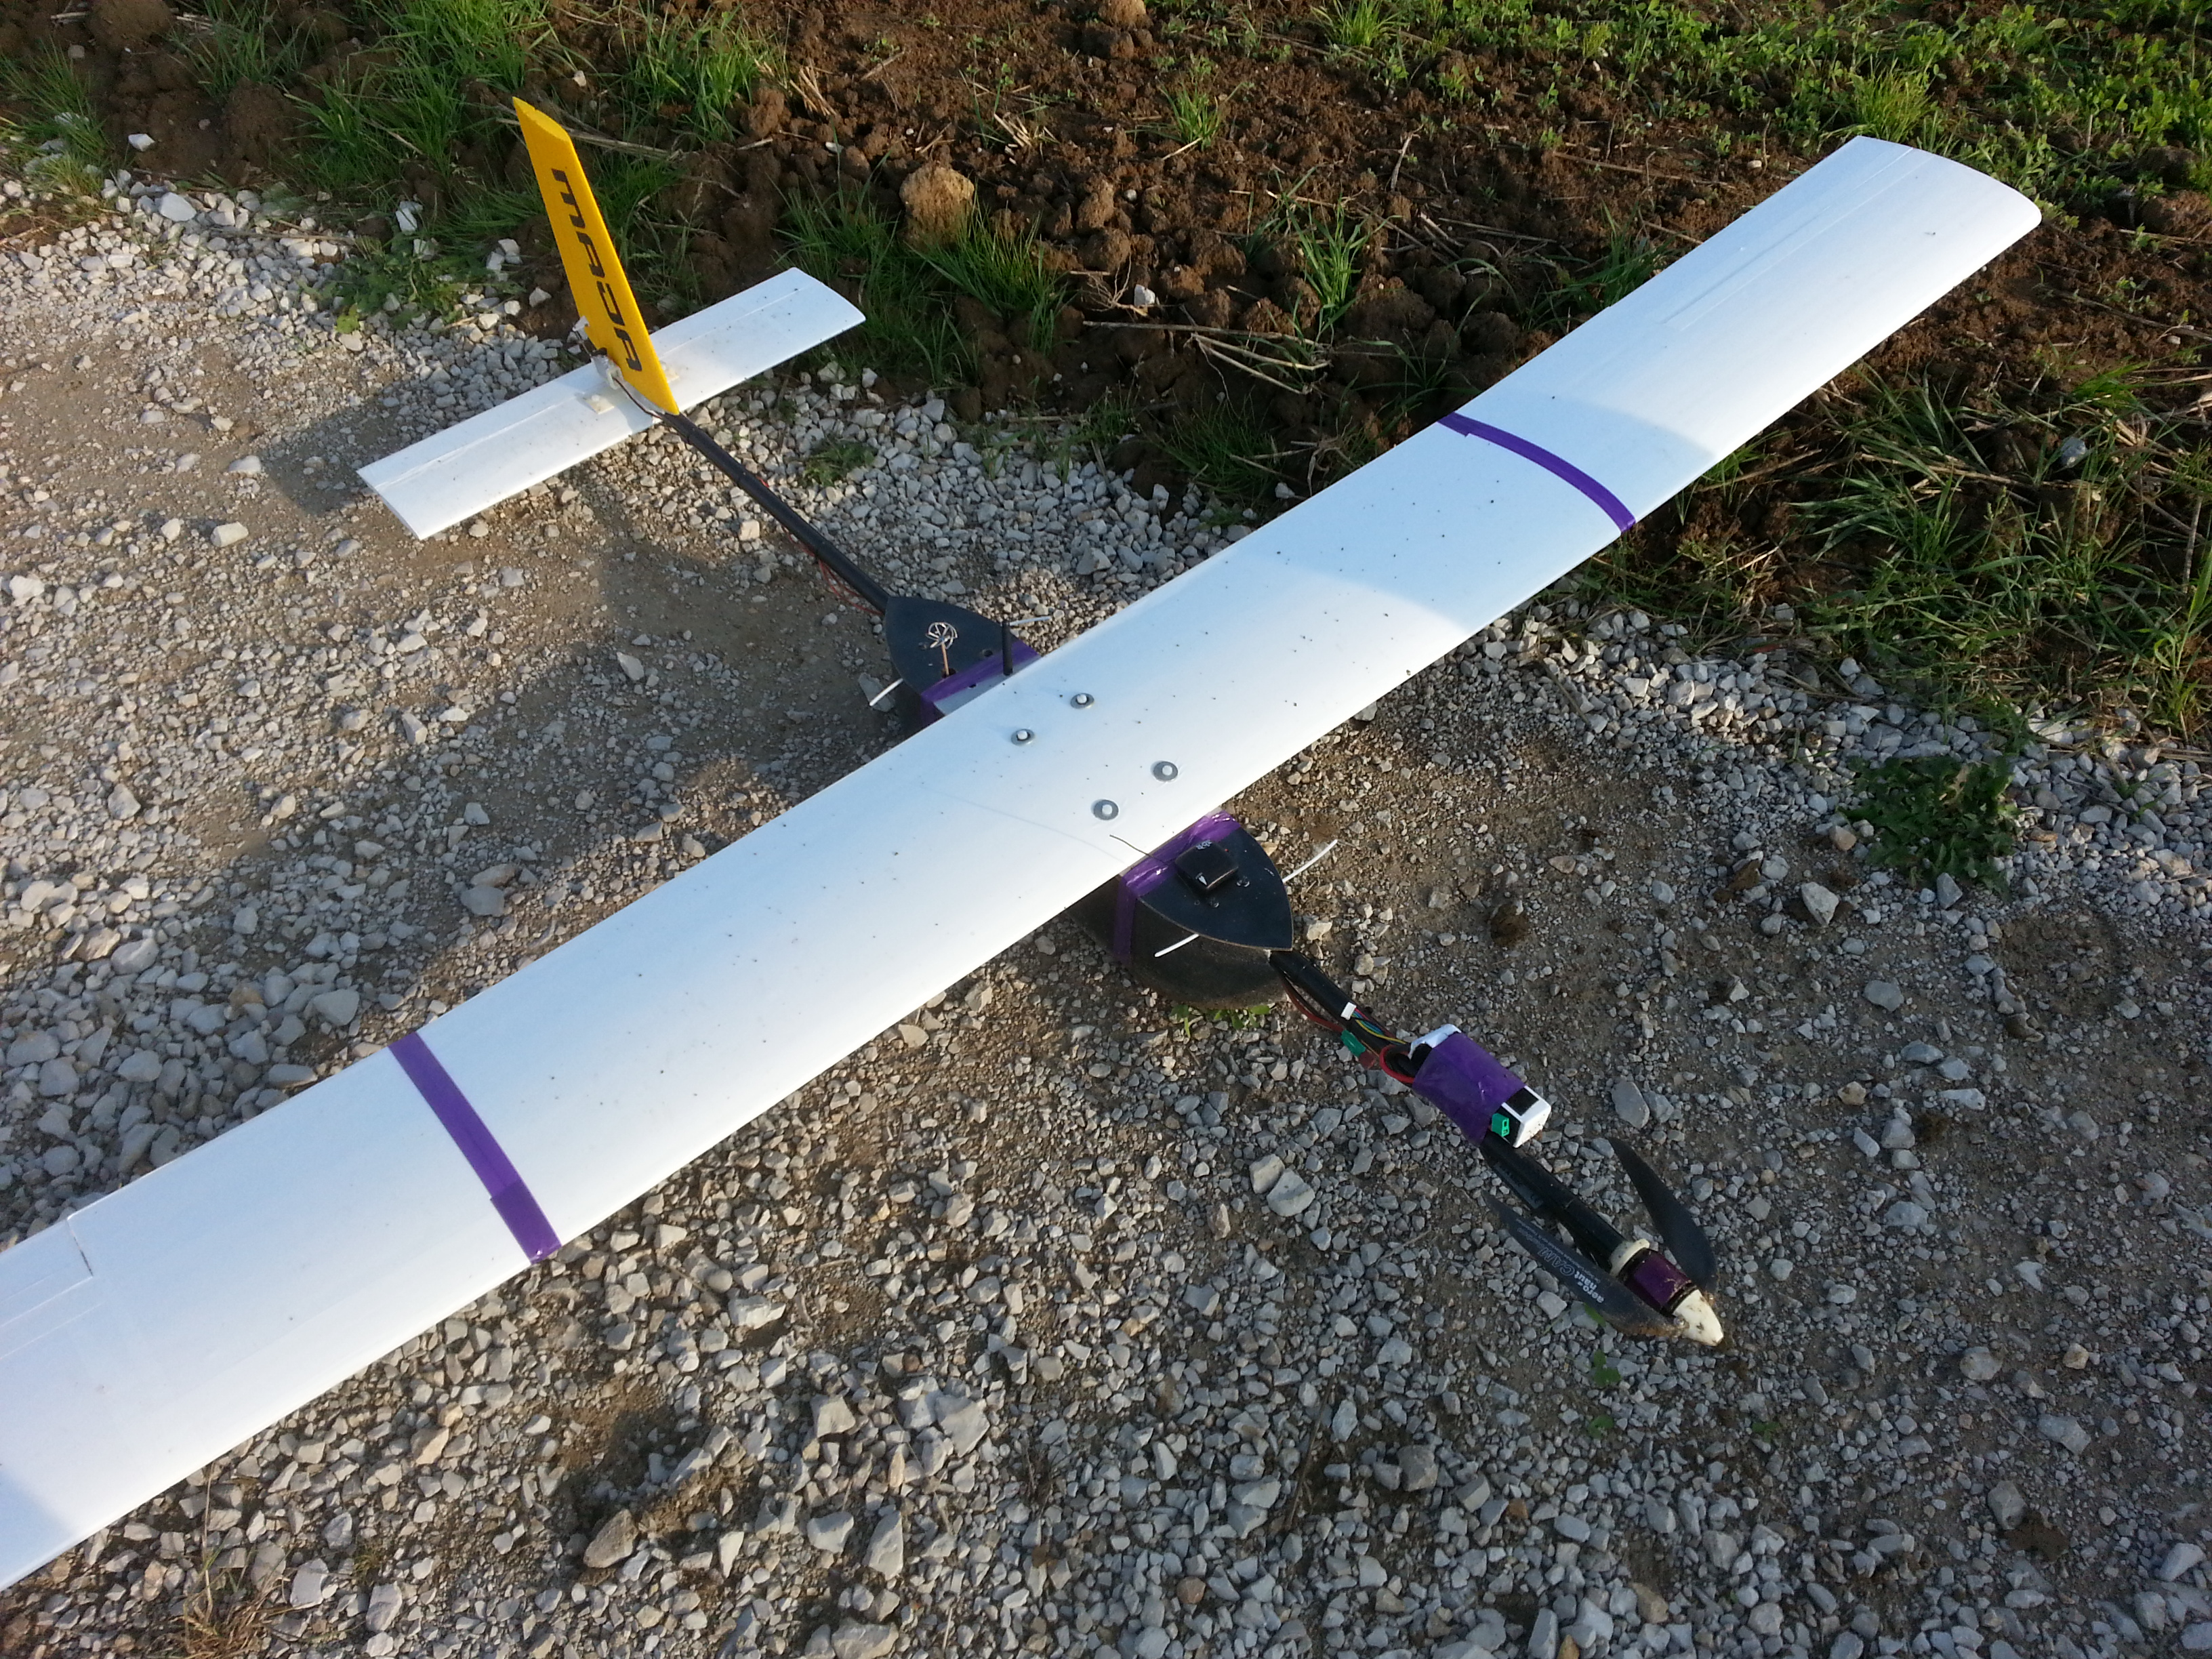
\includegraphics[width=0.9\textwidth]{bilder/Fotos/AUVSI-MAYA-Hybrid.jpg} 
\caption{Frühe Vorversuche für das AUVSI 2015 Flugzeug} 
\label{Frühe Vorversuche für das AUVSI 2015 Flugzeug}
\end{figure}

So entstand im Laufe der Vorbereitung zur ersten Teilnahme am AUVSI SUAS-Wettbewerb 2015 ein voll modulares Hardware Konzept für Flügelkasten, Leitwerk, Leitwerksträger und Nutzlastrumpf. Damit war eine gute Handhabung der einzelnen Sektionen bei der Missionsvorbereitung möglich, durch die modulare Bauweise konnten Modifikationen einfach durchgeführt werden.

Integriert war hier auch die erste Generation einer eigenen Flugzeugbordelektronik für Leistungs- und Signalpfade. Das über zahlreiche Testflüge gereifte Flugsystem konnte so auf dem Wettbewerb einen erfolgreich eingesetzt werden.
\clearpage

\begin{figure}[H]
\centering
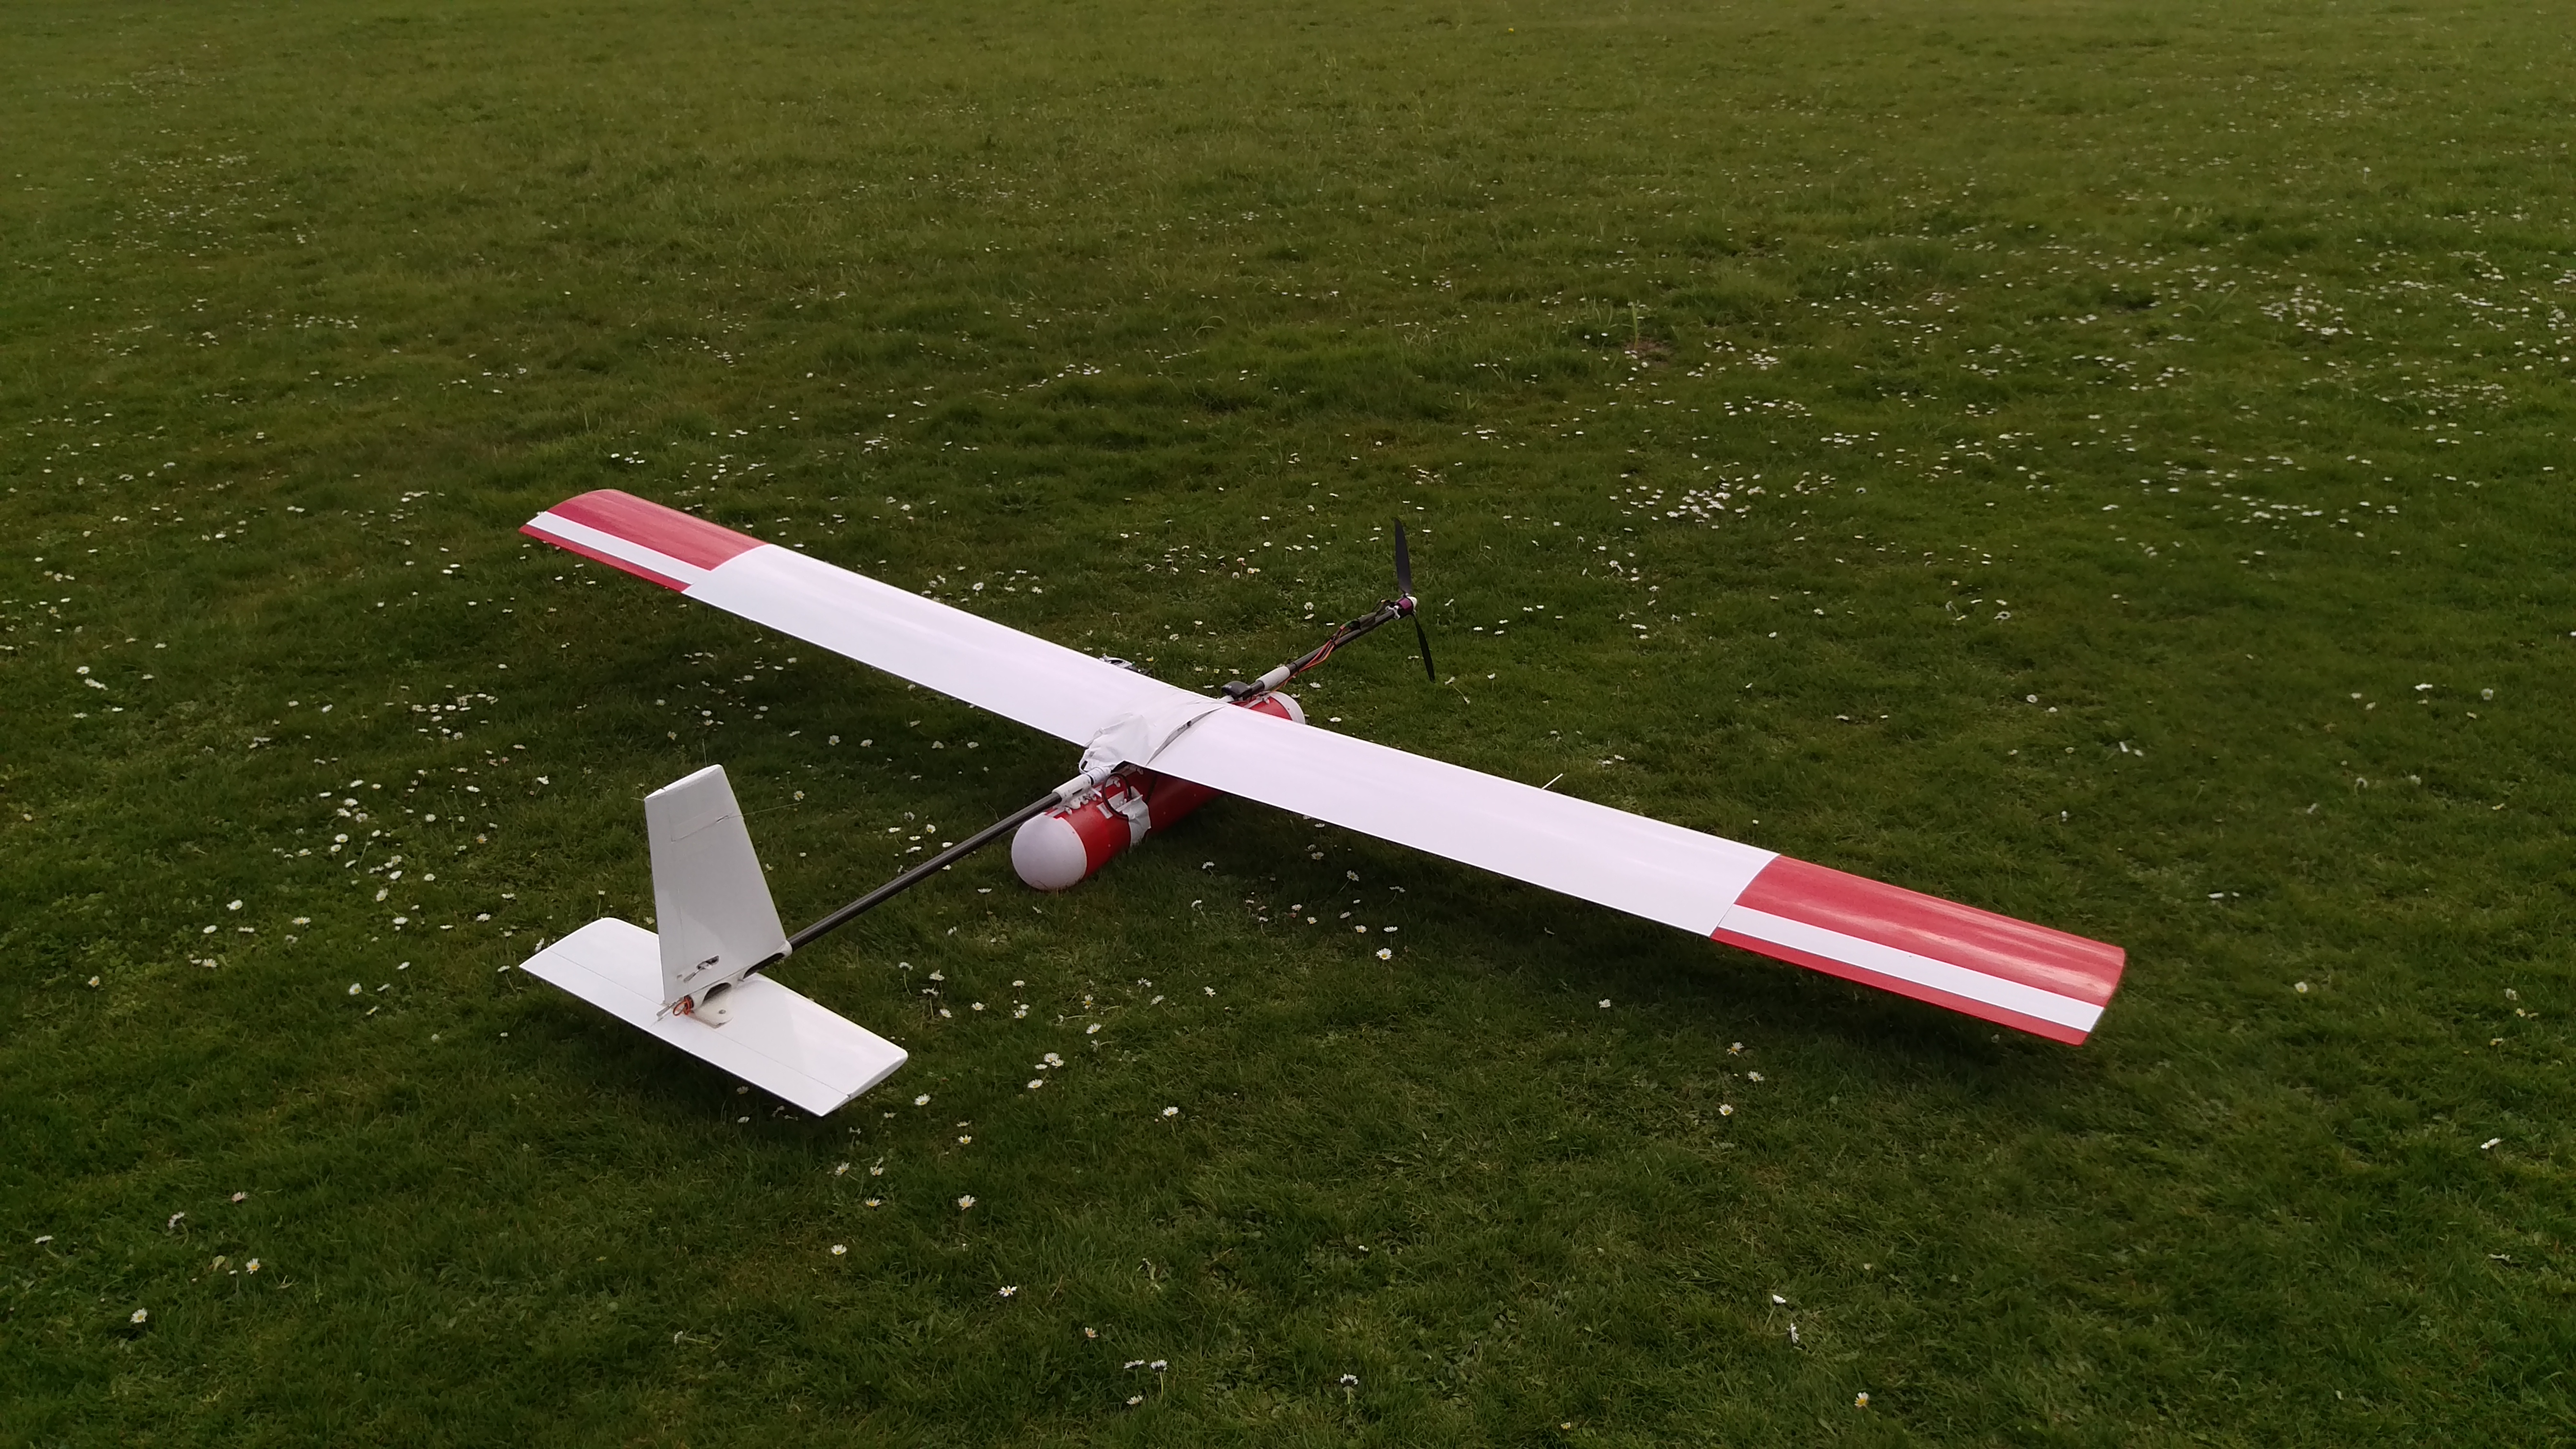
\includegraphics[width=0.9\textwidth]{bilder/Fotos/AUVSI_2015.jpg} 
\caption{Das AUVSI 2015 Modell im Einsatzzustand am Testflugplatz} 
\label{Das AUVSI 2015 Modell in Einsatzzustand am Testflugplatz}
\end{figure}

Im weiteren Verlauf des Jahres 2015 wurde das Forschungs-Kooperationsprojekt mit der Fakultät für Geoinformatik in Angriff genommen. Die bewährte AUVSI SUAS-Wettbewerbs Plattform von 2015 wurde mit einem neuen Nutzlastrumpf nach demselben Modulprinzip versehen, der diesmal eine hochauflösende Spiegelreflexkamara für Reihenbildaufnahmen trug. Hiermit konnten zahlreiche problemlose Missionsflüge im Regenwald von Ecuador durchgeführt werden.

\begin{figure}[H]
\centering
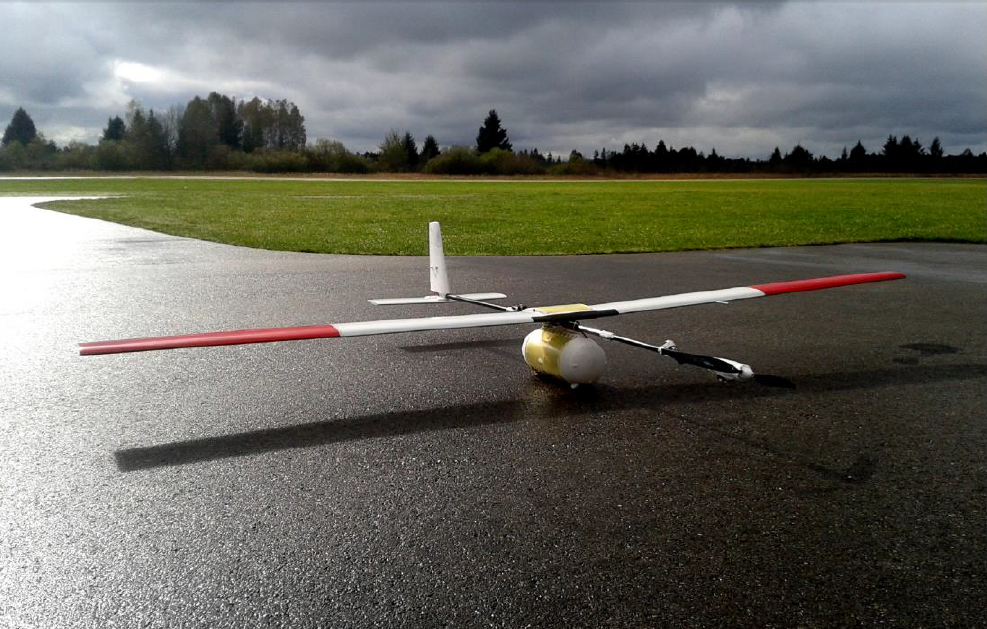
\includegraphics[width=0.9\textwidth]{bilder/Fotos/Ecuadorflieger_Koenigsdorf.png} \caption{Für die Fotomission in Ecuador modifizierter AUVSI 2015 Flieger in Königsdorf} 
\label{Für die Fotomission in Ecuador modifizierter AUVSI 2015 Flieger in Königsdorf}
\end{figure}

\clearpage

\textbf{Wettbewerb 2016:}

Der AUVSI SUAS-Wettbewerbsflieger von 2016 stellt eine konsequente Weiterentwicklung dar,basierend auf den Erfahrungen aus den bisherigen Wettbewerbe und der Ecuador-Mission. Erstmals wurden die Batteriesysteme in die neu gefertigten Flügel verlegt, um Platz im Rumpf zu sparen und die mechanischen Belastungen des Tragwerks zu verringern.

\begin{figure}[H]
\centering
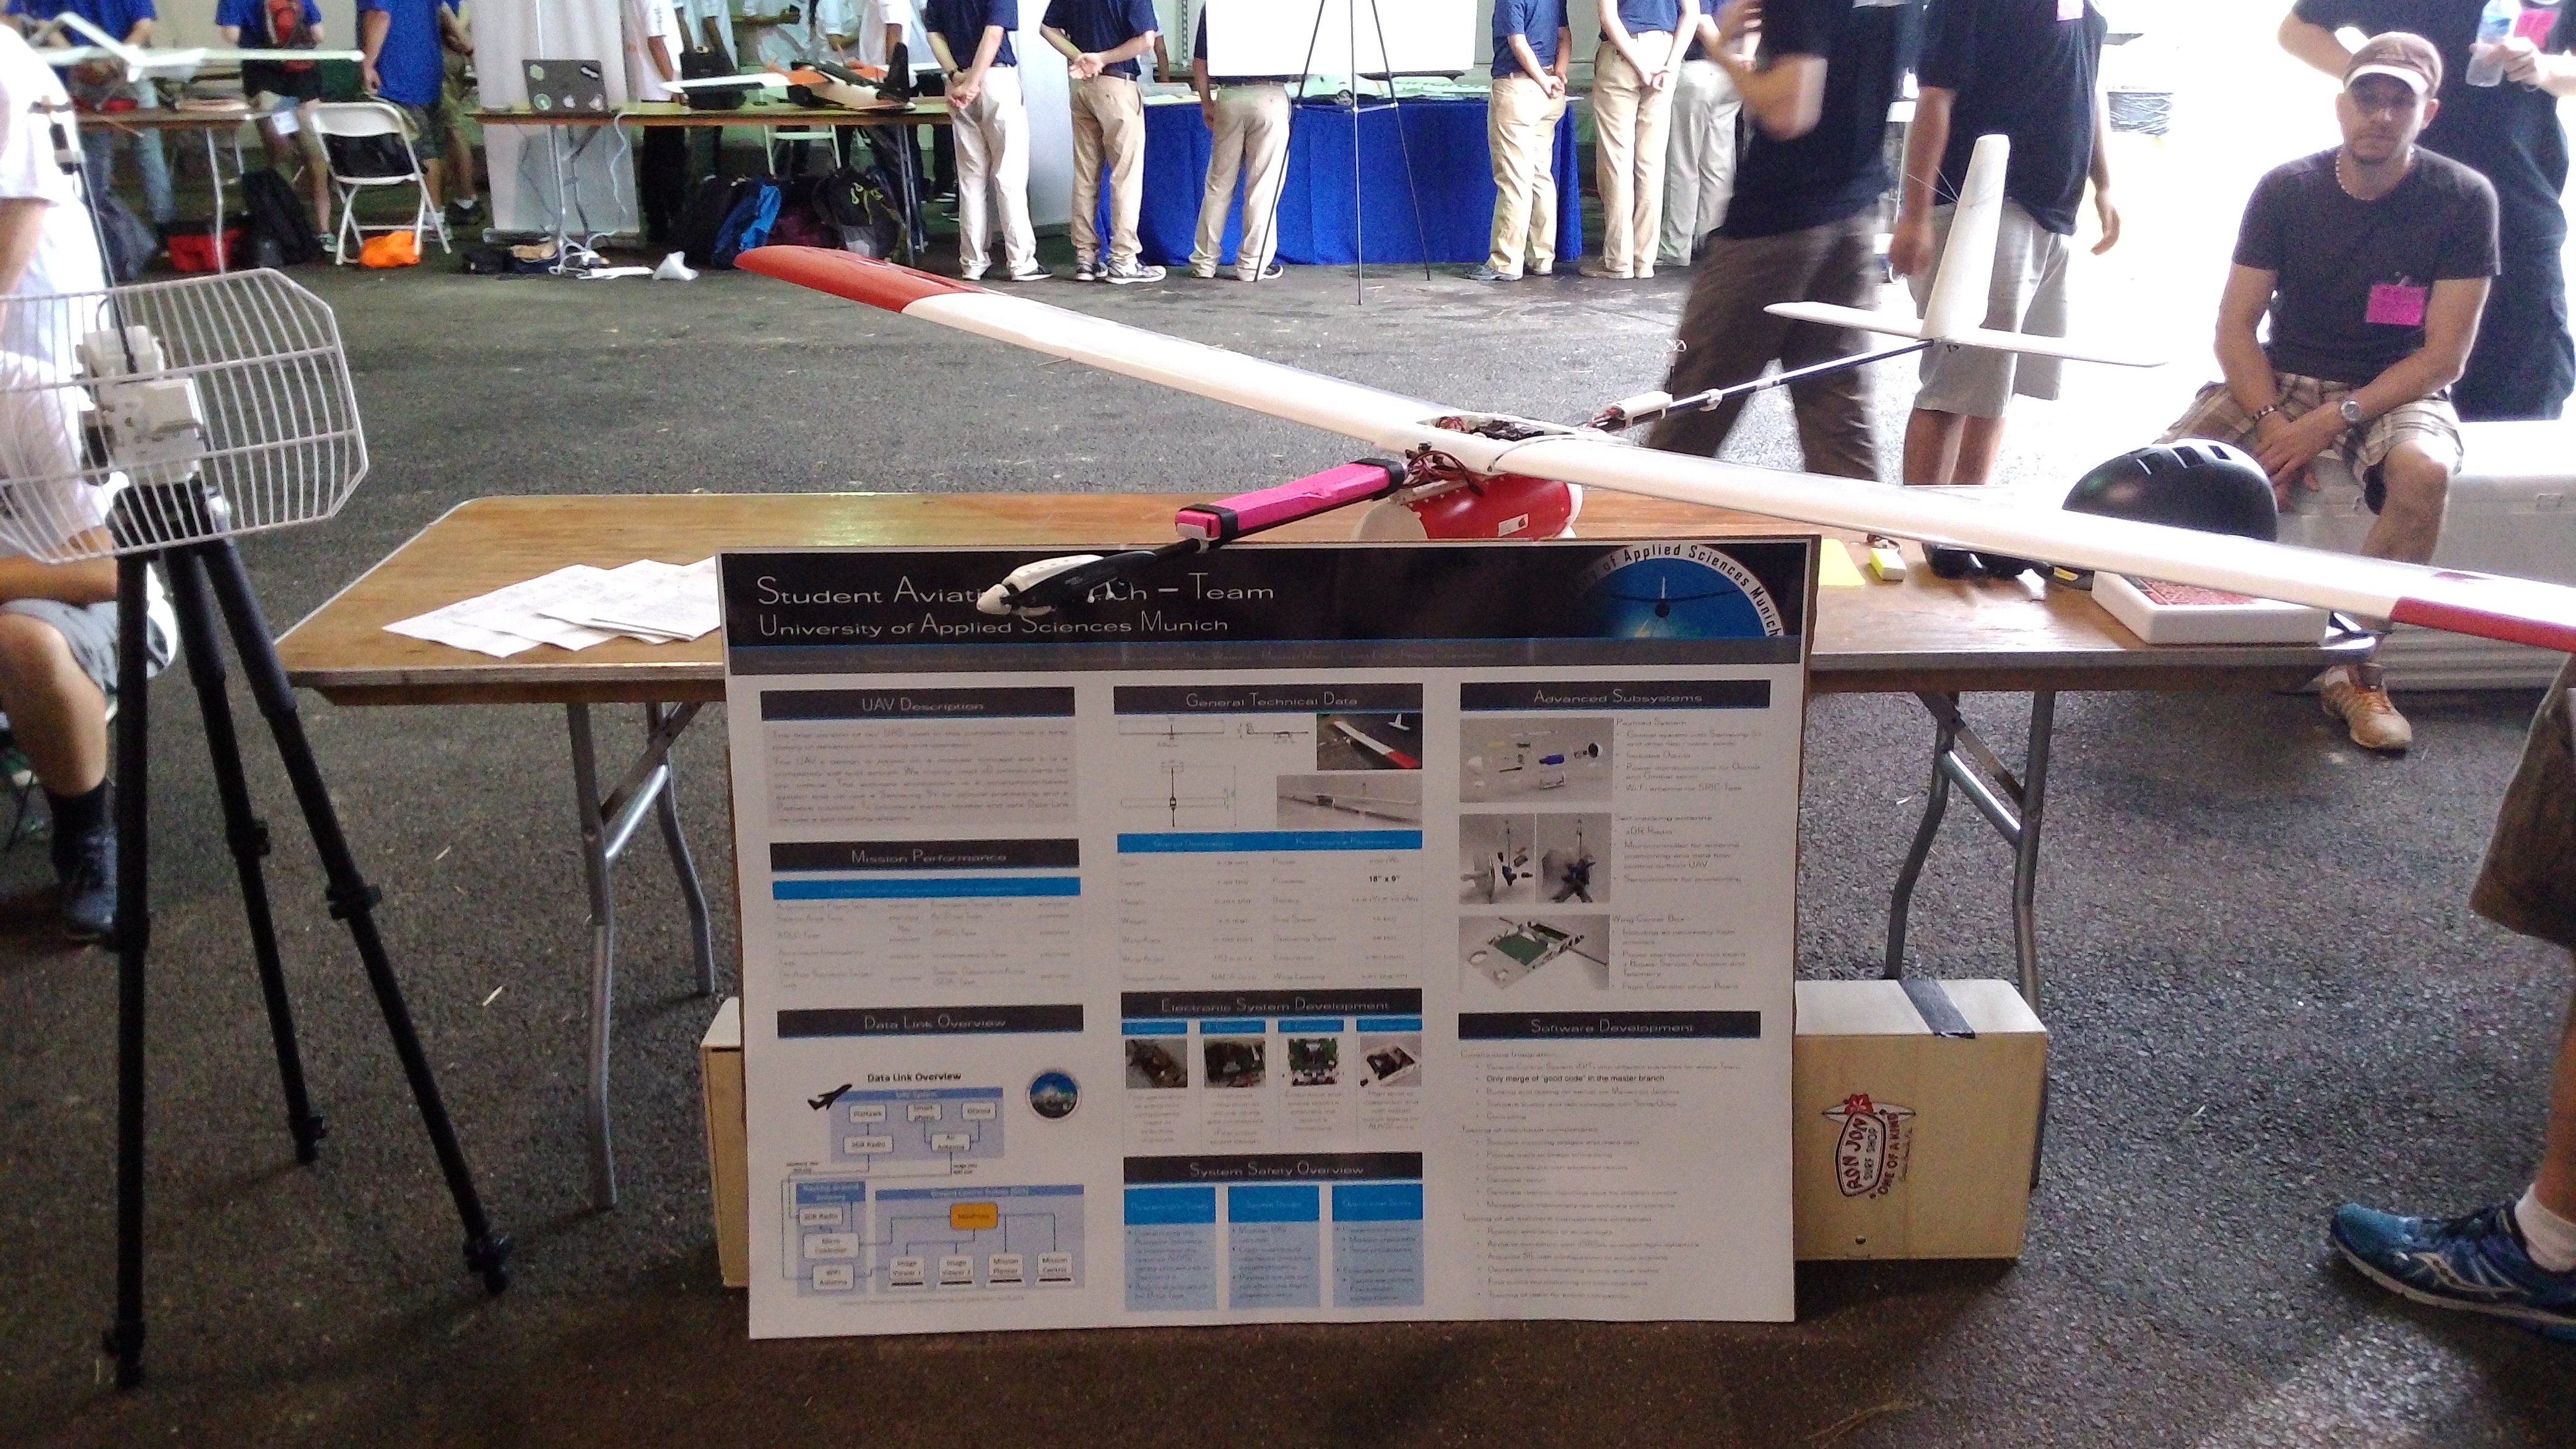
\includegraphics[width=0.9\textwidth]{bilder/Fotos/AUVSI_2016_Display.jpg} 
\caption{Der AUVSI 2016 Flieger bei der Vorstellung auf dem Wettberwerb} 
\label{Der AUVSI 2016 Flieger beim Display auf dem Wettberwerb}
\end{figure}

Eine neue Generation von Bordelektronik ermöglichte die Fremdversorgung des flugbereiten Fliegers beim Warten auf den Start. Die geänderten Anforderungen an zwei Kamerasysteme und den Bordcomputer konnten in einem deutlich verkleinerten Rumpf umgesetzt werden. 





